\section{Future Work}
\label{futurework}

Attractive innovation that could be added into the already existing eclipse plug-in are as follows:

- \textbf{Intent dependencies and options.} Adding additional information to the interface such as code previews, descriptions, a list of required permissions, a list of any required dependencies, and possibly links to documentation, would assist the developer during development. Whilst we currently store permissions and callbacks in our database, the additional information would require modifications to the meta-model and DSL. This information would be included alongside the below list in the plug-in interface.

\begin{figure}[H]
\label{codegeneratorview}
  \centering
    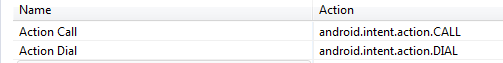
\includegraphics[width=\textwidth]{intentBefore}
  \caption{Future Work 1.0}
\end{figure}

- \textbf{Creating constants and variables}. Many Intents require additional data to perform the call correctly and currently the code generation only inserts pre-defined information as a helper for the developer. A better way of setting this information would be through an interface requesting the user enter the information through the plug-in interface, most probably in a dialog window. This would also resolve the issue that our callback code generation currently has with the variable integer required to detect which call is being returned.

- \textbf{API level support}. Detecting the Android SDK version used, and then modifying the available Intents and code generated for the particular SDK would be a complicated but good feature. This would ensure the code generation works across as many platforms as possible, but compiling the data for each SDK version would be a long and extensive process.

- \textbf{Web-service updates}. Updating the database via a web-service API would ensure the database stays up-to-date and would remove the need to publish new versions of the plug-in when the database should be updated. This would require we setup a server which contains the file but the existing could would remain relatively unchanged, with the only difference being the database file that is loaded.
	